% cmsc351 - Algorithms
%   ██████  ████     ████  ████████   ██████         ████  ██████  ██
%  ██░░░░██░██░██   ██░██ ██░░░░░░   ██░░░░██       █░░░ █░█░░░░  ███
% ██    ░░ ░██░░██ ██ ░██░██        ██    ░░       ░    ░█░█████ ░░██
%░██       ░██ ░░███  ░██░█████████░██        █████   ███ ░░░░░ █ ░██
%░██       ░██  ░░█   ░██░░░░░░░░██░██       ░░░░░   ░░░ █     ░█ ░██
%░░██    ██░██   ░    ░██       ░██░░██    ██       █   ░█ █   ░█ ░██
% ░░██████ ░██        ░██ ████████  ░░██████       ░ ████ ░ ████  ████
%  ░░░░░░  ░░         ░░ ░░░░░░░░    ░░░░░░         ░░░░   ░░░░  ░░░░
%     ██      ██                         ██   ██   ██
%    ████    ░██  █████                 ░░   ░██  ░██
%   ██░░██   ░██ ██░░░██  ██████  ██████ ██ ██████░██      ██████████   ██████
%  ██  ░░██  ░██░██  ░██ ██░░░░██░░██░░█░██░░░██░ ░██████ ░░██░░██░░██ ██░░░░
% ██████████ ░██░░██████░██   ░██ ░██ ░ ░██  ░██  ░██░░░██ ░██ ░██ ░██░░█████
%░██░░░░░░██ ░██ ░░░░░██░██   ░██ ░██   ░██  ░██  ░██  ░██ ░██ ░██ ░██ ░░░░░██
%░██     ░██ ███  █████ ░░██████ ░███   ░██  ░░██ ░██  ░██ ███ ░██ ░██ ██████
%░░      ░░ ░░░  ░░░░░   ░░░░░░  ░░░    ░░    ░░  ░░   ░░ ░░░  ░░  ░░ ░░░░░░
%
\documentclass[english, 10pt]{article}
\usepackage{notes}
\usepackage{inconsolata}
\usepackage[shellescape]{gmp}
\geometry{paperheight=15000pt, left=40pt, top=40pt, textwidth=530pt, marginparsep=20pt, marginparwidth=100pt, textheight=16263pt, footskip=40pt}
\newcommand{\thiscoursecode}{CMSC 351}
\newcommand{\thiscoursename}{Algorithms}
\newcommand{\thisprof}{Dr.\ Clyde Kruskal}
\newcommand{\me}{Alex Reustle}
\newcommand{\thisterm}{Spring 2016}
\newcommand{\website}{http://www.cs.umd.edu/class/spring2016/cmsc351-0101}%chktex 8
\usepackage{ifpdf}
\ifpdf%
\DeclareGraphicsRule{*}{mps}{*}{}
\fi
%%%Headers
\chead{351-Algorithms}
\lhead{\thisterm}

%%%%% TITLE %%%%%
\graphicspath{{../}}
\newcommand{\notefront}{%
\pagenumbering{arabic}
\begin{center}
{\small}
\textbf{\Huge{\noun{\thiscoursecode}}}
{\Huge \par}
{\Large{\noun{\thiscoursename}}}\\
\vspace{0.1in}
\vspace{0in}\includegraphics[scale=0.5]{umd_cs.png} \\
\vspace{0.1in}{\noun\me} \\
{\noun\thisprof} \ $\bullet$ \ {\noun\thisterm} \ $\bullet$ \ {\noun{University of Maryland}} \\
{\ttfamily \url{\website}} \\
\end{center}
}

 \tikzstyle{class}=[
    rectangle,
    draw=black,
    text centered,
    anchor=north,
    text=black,
    text width=2cm,
    shading=axis,
    bottom color={rgb:red,222;green,222;blue,222},
    top color=white,shading angle=45]



%  ██████                   ██
% ░█░░░░██           █████ ░░
% ░█   ░██   █████  ██░░░██ ██ ███████
% ░██████   ██░░░██░██  ░██░██░░██░░░██
% ░█░░░░ ██░███████░░██████░██ ░██  ░██
% ░█    ░██░██░░░░  ░░░░░██░██ ░██  ░██
% ░███████ ░░██████  █████ ░██ ███  ░██
% ░░░░░░░   ░░░░░░  ░░░░░  ░░ ░░░   ░░
\begin{document}
% \renewcommand\familydefault{\sfdefault}
% \sffamily
  % Notes front
  \notefront%
  % Table of Contents and List of Figures
  % \tocandfigures


\section{Maximum Subarray Problem}
Given a sequence of integers, find the largest collection which is a sum of adjacent values.
\[
    3~-5~\underbrace{4~3~-6~4~8}_{Sum = 13}~-5~3~-7~2~1 \\
\]

\subsection{Brute Force solution}
Brute force solution: try every possible sum. (I'd guess it's $n^3$) Sum variable M set to zero. We will allow empty sums (no elements, sum = 0).

% \begin{wrapfigure}{R}{0.3\textwidth}
%     \centering
\begin{algorithm}[H]
$M\gets0$\;
\For{i=1 to n}{\
    \For{j=i to n}{\
        $S\gets0$\;
        \For{k=i to j}{\
            $S = S + A[k]$\;
            $M = \max(M,S)$\;
        }
    }
    \caption{Matrix Subarray Brute Force}
}
\end{algorithm}
% \end{wrapfigure}

Insight: Loops in programs are like summation in Mathematics.%
(for i=1) to n == $\sum_{i=1}^{n}$

Nested loops are nested summations.
$\sum_{i=1}^{n} \sum_{j=i}^{n} \sum_{k=i}^{j} 1$

Simplify summation using summation algebra from the inside out.
$\sum_{i=1}^{n} \sum_{j=i}^{n} j-i+1 $

Tangent: since j is the variable, i and 1 are constants. So it can be separated into two sums.

\subsection{Analysis of the Algorithm}
Actual progress: Change a variable to manage sum. Like integrals in calculus. Every technique in calculus for integrations are matched by similar techniques in summations.
Change of variable by example.
\begin{align*}
    \sum_{i=1}^{n} \sum_{j=i}^{n} \sum_{k=i}^{j} 1 &= \sum_{i=1}^{n} \sum_{j=i}^{n} j-i+1 & \text{By adding 1 $j-i$ times, and fenceposting} \\
    &= \sum_{i=1}^{n} \sum_{j=1}^{n-i+1} j & \text{By change of variable Method} \\
    &= \s{i=1}{n} \f{(n-i+1)(n-i+2)}{2} & \text{Gausses sum} \\
    &= \f{1}{2}\times \s{i=1}{n} (n-i+1)(n-i+2) & \text{Expanding is error prone. Change variable instead} \\
    &= \f{1}{2}\times \s{n-i+1=1}{n} i(i+1) & \text{substitute i=n-i+1} \\
    &= \f{1}{2}\times \s{i=1}{n} i(i+1) & \text{simplify bounds} \\
    &= \f{1}{2}\times \frac{n(n+1)(n+2)}{3} & \text{magic.} \\
    &= \frac{n(n+1)(n+2)}{6} \\
\end{align*}

This first method is $\Theta{\left(n^3\right)}$

\subsection{Methods to improve integer list summation algorithm.}
Remember previous sums, do not recalculate known data.

% \begin{wrapfigure}{L}{0.3\textwidth}
\begin{algorithm}[H]
$M\gets0$\;
\For{i=1 to n}{\
    $S\gets0$\;
    \For{j = i to n}{\
        $S = S+A[i]$\;
        $M = \max(M,S)$\
    }
}
\caption{$n^2$ Subarray }
\end{algorithm}
% \end{wrapfigure}
$$
    \sum_{i=1}^{n} \sum_{j=i}^{n} 1 = \sum_{i=1}^n n-i+1 \\
    = \sum_{i=1}^{n} i = \frac{n(n+1)}{2}
$$
This new method is $\Theta{n^2} $.

% Further improvements.
Loosely speaking the maximum sum is just the previous maximum sum, plus the current value.
% $$
%     S[i] = S[i-1]+A[i] \\
%     \max( S[i-1]+A[i], 0)
% $$

% \begin{wrapfigure}{R}{0.3\textwidth}
\begin{algorithm}[H]
$M \gets 0,S \gets 0$\;
\For{i = 1 to n}{\
    $S \gets \max(S+A[i], 0)$\;
    $M = \max(M,S)$\;
}
\caption{Linear Subarray }
\end{algorithm}
% \end{wrapfigure}

Correctness of the algorithm stems from proof by induction on $S = \max(S+A[i], 0)$. This is the Loop Invariant.

$$
\sum_{i=1}^n 1 = n \\
% \Theta{(n)}
$$

\section{Timing analysis}
\textbf{Lower Bound}

No algorithm is Faster than this boundary condition, the lower bound time.

Best Case scenario, very hard to prove in the general case.

\textbf{Upper Bound}

Some Algorithm can obtain upper bound time.

Worst case Scenario.

\subsection{Classes of algorithms}
\subsubsection{$\Theta(n^2)$}
    Bubble sort \\
    Insertion Sort \\
    Selection Sort \\
\subsubsection{$\Theta(n\log(n))$}
    Merge Sort \\
    Heap Sort \\
    Quick Sort \\
\subsubsection{Others}
    Radix Sort

%% ██████           ██      ██       ██            ████████                   ██
% ░█░░░░██         ░██     ░██      ░██           ██░░░░░░                   ░██
% ░█   ░██  ██   ██░██     ░██      ░██  █████   ░██         ██████  ██████ ██████
% ░██████  ░██  ░██░██████ ░██████  ░██ ██░░░██  ░█████████ ██░░░░██░░██░░█░░░██░
% ░█░░░░ ██░██  ░██░██░░░██░██░░░██ ░██░███████  ░░░░░░░░██░██   ░██ ░██ ░   ░██
% ░█    ░██░██  ░██░██  ░██░██  ░██ ░██░██░░░░          ░██░██   ░██ ░██     ░██
% ░███████ ░░██████░██████ ░██████  ███░░██████   ████████ ░░██████ ░███     ░░██
% ░░░░░░░   ░░░░░░ ░░░░░   ░░░░░   ░░░  ░░░░░░   ░░░░░░░░   ░░░░░░  ░░░       ░░

\section{Bubble Sort Analysis}
\begin{algorithm}
\For{i = n downto 2}{%
    \For{j = 1 to i-1}{%
        \If{$A[j] > A[j+i]$}{%
        swap (A[j],A[j+1])\;
        }
    }
    \caption{Bubble Sort}
}
\end{algorithm}

Major Growth Elements of Bubble sort will be Comparisons and Exchanges.\\

Best case number of comparisons require you to view every element unconditionally. \\
\begin{align*}
    \sum_{i=2}^n \sum_{j=1}^{i-1} &= \sum_{i=2}^{n} i-1 \\
    &= \sum_{i=1}^{n-1} (i+1) -1 \\
    &= \sum_{i=1}^{n-1} i \\
    &= \f{(n-1)n}{2}
\end{align*}
Comparisons will always occur, regardless of state of list. \\

Best Case Exchanges occur when the list is sorted. Zero exchanges. \\
Worst Case Exchanges occur when the list is reverse sorted. Same number of exchanges as comparisons. \\

\defn[Random] Each permutation (ordering) of the list is equally likely.

    Rotations of list permutations are equally likely to be in any position, but are not random because they ignore other possible permutations.\\

\subsection{Average Case Analysis}
Count Transpositions. Two elements that are out of order related to each other. \\

In the best case there are no transpositions. \\
In the worst case there are n choose 2 transpositions. Every element is out of order with the number of elements below it.
So the number of transpositions is the number of unique pairs. Which is n choose 2 pairs. \\
In a randomized sample the permutations are equally likely to be out of order greater or lesser,
so the number of average case exchanges will be half the number of comparisons. $\f{n(n-1)}{4}$.


 % ██                                   ██   ██                      ████████                   ██
% ░██                                  ░██  ░░                      ██░░░░░░                   ░██
% ░██ ███████   ██████  █████  ██████ ██████ ██  ██████  ███████   ░██         ██████  ██████ ██████
% ░██░░██░░░██ ██░░░░  ██░░░██░░██░░█░░░██░ ░██ ██░░░░██░░██░░░██  ░█████████ ██░░░░██░░██░░█░░░██░
% ░██ ░██  ░██░░█████ ░███████ ░██ ░   ░██  ░██░██   ░██ ░██  ░██  ░░░░░░░░██░██   ░██ ░██ ░   ░██
% ░██ ░██  ░██ ░░░░░██░██░░░░  ░██     ░██  ░██░██   ░██ ░██  ░██         ░██░██   ░██ ░██     ░██
% ░██ ███  ░██ ██████ ░░██████░███     ░░██ ░██░░██████  ███  ░██   ████████ ░░██████ ░███     ░░██
% ░░ ░░░   ░░ ░░░░░░   ░░░░░░ ░░░       ░░  ░░  ░░░░░░  ░░░   ░░   ░░░░░░░░   ░░░░░░  ░░░       ░░
\section{Insertion Sort}

Every 0 to [i-1] index during the loop will be sorted. \\
ith term is stored in tmp. Values in the sorted subarray which are larger than the tmp value are brought forward individually until tmp > A[j]. \\

\begin{algorithm}
$A[0] \gets -\infty$\;
\For{i = 2 to n}{%
    $t \gets A[i]$\;
    $j =i-1$\;
    \While{$A[j] \ge t$}{%
        $A[j+1] \gets A[j]$\;
        $j{-}{-}$\;
    }
    $A[j+1] \gets t$\;
}
\caption{Insertion Sort}
\end{algorithm}

\subsection{Analysing Number of Comparisons}

\subsubsection{Best Case Comparisons}
In the case where the array is already correctly sorted, there will be only 1 comparison for each iteration of the other for loop.
It will always evaluate false.
So the number of best case comparisons is just the number of for loop iterations.
\begin{align*}
    \s{i=2}{n} 1 &= (n-2)+1 & \text{Already sorted} \\
    &= n-1
\end{align*}

\subsubsection{Worst Case Comparisons}
In the worst case the array is reverse sorted, and every element must be moved.
The while loop always decrements j to zero to compare against the sentinel value.
\begin{align*}
    \sum_{i=2}^n i &= \left(\sum_{i=1}^{n}i \right)-1 & \text{Reverse Sorted} \\
    &= \f{n(n+1)}{2} -1 & \text{must remove i=1} \\
    &= \f{(n+2)(n-1)}{2}
\end{align*}

\subsubsection{Average Case Comparisons}
In the average case we must determine the probability that a given element will move.
So for evaluation we want the expected value over the set $\sum_{x \in X} P(x)\cdot V(x) $.

Starting at location i, go until reach location j-1.
Probability that 1 element (A[i]) will end up in any location in the subarray is $\f{1}{i}$
Value is number of moves. Which is (i-j+1).

\begin{align*}
    \s{i=2}{n} \s{j=1}{i} \frac{1}{i} \cdot (i-j+1) &= \s{i=2}{n} \frac{1}{i} \s{j=1}{i} (i-j+1)  &  \text{Pull out 1/i} \\
 &= \s{i=2}{n}\frac{1}{i}\s{j=1}{i} j \\
 &= \s{i=2}{n}\frac{1}{i}\cdot\frac{i(i+1)}{2} \\
 &= \s{i=2}{n}\frac{(i+1)}{2} \\
 &= \frac{1}{2}\left[ \s{i=2}{n}i+1\right] \\
 &= \frac{1}{2}\left[ \s{i=2}{n}i+ \s{i=2}{n}1\right] \\
 &= \frac{1}{2}\left[ \s{i=1}{n}i -1 + (n-1) \right] \\
 &= \frac{1}{2}\left[ \f{(n)(n+2)}{2} -1 + \frac{2(n-1)}{2} \right] \\
 &= \frac{1}{2}\left[ \f{(n^2+n-2)}{2} + \frac{2n-2}{2} \right] \\
 &= \f{(n^2+3n-4)}{4}  \\
 &= \f{(n+4) (n-1)}{4}
\end{align*}


\subsection{Analyzing Exchanges}

\subsubsection{Best Case Exchanges}
Best case number of moves = $2n-1$. There is 1 move in in the $-\infty$ assignment at the top, then in the for loop there are 2 moves per iteration, moving A[i] into t,
and moving it back into the same spot. $1 + 2(n-1) = 2n -1$. \\

\subsubsection{Worst Case Exchanges}
Worst case number of moves is 2 for each iteration of outer loop plus worst case number of comparisons, minus the time when the comparison is false at the end, of the inner loop, plus 1 for the top assignment. $2(n-1) + COMP - (n-1) +1 $.

Note the short cut, at each iteration we're doing one more move than comparison. So just easily take the value already derived for Worst case comparisons,
and add the number of loop iterations, plus 1 for the sentinel assignment.
$$\frac{(n+2)(n-1)}{2} +n $$

\subsubsection{Average Case Exchanges}
In the average case, whenever there's a comparison, there will always be a move, except the 1 time per iteration it evaluates false.
So the analysis method is the same as for the worse case. Since we know the number.
$$\f{(n+4) (n-1)}{4} + n$$
\begin{rem}
An important trick is to recognize that the moves are related to the comparisons 1 to 1 and that there will be 1 time when the comparison evaluates false each iteration, so you subtract that from the final analysis.
\end{rem}


%  ██                                   ██   ██                      ████████                   ██                      ██
% ░██                                  ░██  ░░                      ██░░░░░░                   ░██                     ██
% ░██ ███████   ██████  █████  ██████ ██████ ██  ██████  ███████   ░██         ██████  ██████ ██████   ███     ██     ██    ██████
% ░██░░██░░░██ ██░░░░  ██░░░██░░██░░█░░░██░ ░██ ██░░░░██░░██░░░██  ░█████████ ██░░░░██░░██░░█░░░██░   ░░██  █ ░██    ██    ██░░░░██
% ░██ ░██  ░██░░█████ ░███████ ░██ ░   ░██  ░██░██   ░██ ░██  ░██  ░░░░░░░░██░██   ░██ ░██ ░   ░██     ░██ ███░██   ██    ░██   ░██
% ░██ ░██  ░██ ░░░░░██░██░░░░  ░██     ░██  ░██░██   ░██ ░██  ░██         ░██░██   ░██ ░██     ░██     ░████░████  ██     ░██   ░██
% ░██ ███  ░██ ██████ ░░██████░███     ░░██ ░██░░██████  ███  ░██   ████████ ░░██████ ░███     ░░██    ███░ ░░░██ ██      ░░██████
% ░░ ░░░   ░░ ░░░░░░   ░░░░░░ ░░░       ░░  ░░  ░░░░░░  ░░░   ░░   ░░░░░░░░   ░░░░░░  ░░░       ░░    ░░░    ░░░ ░░        ░░░░░░
%   ████████                    ██   ██                   ██
%  ██░░░░░░                    ░██  ░░                   ░██
% ░██         █████  ███████  ██████ ██ ███████   █████  ░██
% ░█████████ ██░░░██░░██░░░██░░░██░ ░██░░██░░░██ ██░░░██ ░██
% ░░░░░░░░██░███████ ░██  ░██  ░██  ░██ ░██  ░██░███████ ░██
%        ░██░██░░░░  ░██  ░██  ░██  ░██ ░██  ░██░██░░░░  ░██
%  ████████ ░░██████ ███  ░██  ░░██ ░██ ███  ░██░░██████ ███
% ░░░░░░░░   ░░░░░░ ░░░   ░░    ░░  ░░ ░░░   ░░  ░░░░░░ ░░░

\section{Insertion Sort without Sentinel}

Add another comparison in the algorithm so the A[0] term is unnecessary, by checking that you haven't gone past i=1.

\begin{algorithm}[H]
    \For{i=2 to n}{%
        $t\gets A[i]$\;
        $j=i-1$\;
        \While{$j > 0 \wedge A[j] > t$}{%
            $A[j+1]\gets A[j]$\;
            $j{-}{-}$\;
        }
        $A[j+1]\gets t$\;
    }
\caption{Insertion Sort w/o Sentinel}
\end{algorithm}

A note about comparisons. We don't count index value comparisons, because index values can easily be stored in registers and won't have the same
cost to check as array value comparisons.

\subsection{Best Case Comparisons}
In the best case, the array is already sorted, so there will just be 1 comparison per iteration of the outer loop. $\s{i=2}{n} 1 = n-1$

\subsection{Worst Case Comparisons}
In the worst case the array is reverse sorted, and every ith iteration of the loop must compare against all previous elements.
\begin{align*}
    \s{i=2}{n}\s{j=1}{i}1 &= \s{i=2}{n} i-1 \\
    &= \s{i=2}{n} i - \s{i=2}{n} 1 \\
    &= \f{n(n+1)}{2} -1 -(n-1) \\
    &= \f{n(n+1)}{2} -n \\
    &= \f{n^2 + n}{2} -\frac{2n}{2} \\
    &= \f{n^2 - n}{2} \\
    &= \f{n(n-1)}{2} \\
\end{align*}
% $$\frac{n(n-1)}{2}$$


\subsection{Average Case Comparisons}
\begin{rem}
HARMONIC SERIES and brick problem.
How far out can you stack bricks on top of one another? Arbitrarily far out (but not infinitely far out)
$$H_n = \s{i=1}{n}\frac{1}{i} = 1+\frac{1}{2}+\frac{1}{3}+\frac{1}{4}+\frac{1}{5}+\cdots \approx \ln{n}+1$$
$$H_n -1 = \s{i=2}{n}\frac{1}{i} = \frac{1}{2}+\frac{1}{3}+\frac{1}{4}+\frac{1}{5}+\cdots \approx \ln{n}$$
Harmonic Series come up again and again because of the idea that something has a$ \frac{1}{i}$ chance of happening in an iteration.
\end{rem}
What are we saving when we don't have a sentinel? In the event that the ith element is the smallest element in the A[1..i-1] sub-array, we will descend all
the way to the 1st index of the list. If that happens, we won't have the 1 extra step of comparing against the sentinel. So only when the ith element is
the smallest seen thus far do we save 1 step.
Probability that current ith element is smallest in sub array is $\frac{1}{i}$. The value when that occurs is 1.
Thus over all n elements of the array, on average the sentinel would have cost us $\s{i=2}{n}\frac{1}{i} = H_n -1$ comparisons.

So average Case comparisons without sentinel is average case with sentinel minus average cost of sentinel.
$\frac{(n-1)(n+4)}{4}-(H_n -1) \approx \frac{(n-1)(n+4)}{4}-\ln{n}$.

\subsection{Exchanges}
Removing the sentinel from insertion sort adds no new exchanges, nor does it alter when a change might have been done already.
Best, worst and average cases are all the same, therefore.


%   ████████          ██                   ██   ██                      ████████                   ██
%  ██░░░░░░          ░██                  ░██  ░░                      ██░░░░░░                   ░██
% ░██         █████  ░██  █████   █████  ██████ ██  ██████  ███████   ░██         ██████  ██████ ██████
% ░█████████ ██░░░██ ░██ ██░░░██ ██░░░██░░░██░ ░██ ██░░░░██░░██░░░██  ░█████████ ██░░░░██░░██░░█░░░██░
% ░░░░░░░░██░███████ ░██░███████░██  ░░   ░██  ░██░██   ░██ ░██  ░██  ░░░░░░░░██░██   ░██ ░██ ░   ░██
%        ░██░██░░░░  ░██░██░░░░ ░██   ██  ░██  ░██░██   ░██ ░██  ░██         ░██░██   ░██ ░██     ░██
%  ████████ ░░██████ ███░░██████░░█████   ░░██ ░██░░██████  ███  ░██   ████████ ░░██████ ░███     ░░██
% ░░░░░░░░   ░░░░░░ ░░░  ░░░░░░  ░░░░░     ░░  ░░  ░░░░░░  ░░░   ░░   ░░░░░░░░   ░░░░░░  ░░░       ░░

\section{Selection Sort}
Summary: Find biggest element, put at bottom of list, recurse for sub array.

\begin{algorithm}[H]
    \For{i=n downto 2}{%
        $k\gets 1$\;
        \For{j=2 to i}{%
            \If{$A[j] > A[k]$}{%
                $k \gets j$\;
            }
        }
        swap (A[k], A[i])\;
    }
    \caption{Selection Sort}
\end{algorithm}

\subsection{Best Case Comparisons}
The comparison is always run, so the comparison value should be the same for each case.
\begin{align*}
    \s{i=2}{n}\s{j=2}{i}1 &= \s{i=2}{n} (i-1) \\
    & = \frac{(n-1)n}{2}\\
\end{align*}

\subsection{Exchanges}
Exchanges don't occur inside the conditional, so exchanges number is simply n-1.

How many times do we exchange a number with itself? How many times does i=k?
$\sum 1/i = H_n$



 % ████     ████                                   ████████                   ██
% ░██░██   ██░██                 █████            ██░░░░░░                   ░██
% ░██░░██ ██ ░██  █████  ██████ ██░░░██  █████   ░██         ██████  ██████ ██████
% ░██ ░░███  ░██ ██░░░██░░██░░█░██  ░██ ██░░░██  ░█████████ ██░░░░██░░██░░█░░░██░
% ░██  ░░█   ░██░███████ ░██ ░ ░░██████░███████  ░░░░░░░░██░██   ░██ ░██ ░   ░██
% ░██   ░    ░██░██░░░░  ░██    ░░░░░██░██░░░░          ░██░██   ░██ ░██     ░██
% ░██        ░██░░██████░███     █████ ░░██████   ████████ ░░██████ ░███     ░░██
% ░░         ░░  ░░░░░░ ░░░     ░░░░░   ░░░░░░   ░░░░░░░░   ░░░░░░  ░░░       ░░
\section{Merge Sort}
Divide and Conquer. Recursively split array down to 1, then merge sorted sublists.
First call of Mergesort is (A,1,n) \\


\begin{algorithm}[H]
    MERGESORT (A,p,r)\;
    //p and r are indecies in array defining sub array.\;
    \If{p<r}{%
        $q \gets \lfloor{\frac{p+r}{2}}\rfloor$\;
        MERGESORT (A,p,q)\;
        MERGESORT (A,q+1,r)\;
        MERGE (A, (p,q), (q+1,r))\;
    \caption{Merge Sort}
    }
\end{algorithm}


\subsection{Merge Comparison analysis}
\subsubsection{Equal length arrays}
Merge algorithm is linear over 2 sorted lists of same size. Total number of comparisons in the worst case during merge is $2n-1$, best case comparisons is n, where
1 array is strictly greater than the other.

Can't do better than $2n-1$ in worst case, because worst case situation is 2 lists with interleaved values. In this case the granularity of difference is on the scale of 1 value. So you must check every value to ensure against that.

This gives us very tight bounds and lets us know everything there is to know about merging.

\subsubsection{Different length arrays}
Arrays of size m and n where $m\le n$ Worst case comparisons = $m+n-1$

When $m<<n$ you can get close to $\log n$ running time using binary search. But when m is close to n you are much closer to the $m+n-1$ worst case.


\subsection{Mergesort Comparison Analysis}
\textbf{Exact Number of Comparisons During a merge}
$$ (q-p+1) + (r-(q+1)+1) -1 = (r-p)\; \text{comparisons} $$
starting at index p and ending at index q. So for the full list, where p=1 and q=n a MERGESORT will start with (n-1) comparisons and have the following behavior.

\begin{tikzpicture}[level/.style={sibling distance=55mm/#1, level distance = 1.5cm}]
\node  (z){$n-1$}
    child {node  (1a) {$\frac{n}{2}-1$}
        child {node  (2a) {$\frac{n}{2^2}-1$}
            child {node {$\vdots$}
                child {node  (3a) {$\left(\frac{n}{2^k}-1\right)$}
                    child {node  (01) {0}}
                    child {node  (02) {0}}
                }
                child {node  (3b) {$\left(\frac{n}{2^k}-1\right)$}
                    child {node  (03) {0}}
                    child {node  (04) {0}}
                }
            }
            child {node {$\vdots$}}
        }
        child {node  (2b) {$\frac{n}{2^2}-1$}
            child {node {$\vdots$}}
            child {node {$\vdots$}}
        }
    }
    child {node  (1b) {$\frac{n}{2}-1$}
        child {node  (2c) {$\frac{n}{2^2}-1$}
            child {node {$\vdots$}}
            child {node {$\vdots$}}
        }
        child {node  (2d) {$\frac{n}{2^2}-1$}
            child {node {$\vdots$}}
            child {node {$\vdots$}
                child {node  (3c) {$\left(\frac{n}{2^k}-1\right)$}}
                child {node  (3d) {$\left(\frac{n}{2^k}-1\right)$}
                    child{node (05) {0}}
                    child{node (06) {0}
                        child [grow=right] {node (eq0) {$=$} edge from parent[draw=none]
                            child [grow=right] {node (eq0) {$0n$} edge from parent[draw=none]
                                child [grow=up] {node (eq1) {$2^k \left( \frac{n}{2^k}-1 \right)$} edge from parent[draw=none]
                                      child [grow=up] {node (eq2) {$\vdots$} edge from parent[draw=none]
                                          child [grow=up] {node (eq3) {$2^2 \left( \frac{n}{2^2}-1 \right)$} edge from parent[draw=none]
                                              child [grow=up] {node (eq4) {$2\left( \frac{n}{2}-1 \right)$} edge from parent[draw=none]
                                                  child [grow=up] {node (eq5) {$n-1$} edge from parent[draw=none]}
                                      }
                                    }
                                  }
                                }
                            child [grow=down] {node (eq6) {$\s{i=0}{\lg n} 2^i (\frac{n}{2^i}-1)$}edge from parent[draw=none]}
                            }
                        }
                    }
                }
            }
        }
};
\path (1a) -- (1b) node [midway] {+};
\path (2a) -- (2b) node [midway] {+};
\path (2b) -- (2c) node [midway] {+};
\path (2c) -- (2d) node [midway] {+};
\path (3a) -- (3b) node [midway] {+};
\path (3c) -- (3b) node (3cent) [midway] {+};
\path (3c) -- (3cent) node (3cent) [midway] {$\cdots$};
\path (3cent) -- (3a) node (3cent) [midway] {$\cdots$};
\path (3c) -- (3d) node [midway] {+};
\path (01) -- (02) node [midway] {+};
\path (03) -- (04) node [midway] {+};
\path (05) -- (06) node [midway] {+};
\path (01) -- (06) node (0cent) [midway] {+};
\path (0cent) -- (05) node [midway] {$\cdots$};
\path (0cent) -- (02) node [midway] {$\cdots$};
\path (eq0) -- (eq1) node [midway] {+};
\path (eq2) -- (eq1) node [midway] {+};
\path (eq2) -- (eq3) node [midway] {+};
\path (eq4) -- (eq3) node [midway] {+};
\path (eq5) -- (eq4) node [midway] {+};
\path (eq0) -- (eq6) node [midway] {=};
\end{tikzpicture}


Because this gives $\lg n$ terms, we can make it a little easier by dropping the bottom row, which sums to 0 anyway, because it's $0n$.
\begin{align*}
    \s{i=0}{\lg(n-1)} 2^i (\frac{n}{2^i}-1) &= \s{i=0}{\lg(n-1)} (n-2^i) \\
    &= \s{i=0}{\lg(n-1)} n - \s{i=0}{\lg(n-1)} 2^i \\
    &= (n\lg(n)) - (2^{\lg(n-1)+1} -1) & \text{geometric series} \\
    &= (n\lg(n)) - (n-1) \\
    &= n\lg(n) - n+1 \\
\end{align*}

\subsection{Merge Sort Recurrence}
When expressed as a recurrence relation, the mergesort algorithm given previously behaves like
\begin{align*}
    S(n) &= S\left( \frac{n}{2} \right)+S\left( \frac{n}{2} \right)+n-1 \\
    &= 2\cdot S\left( \frac{n}{2} \right)+n-1 \\
    \intertext{Which gives the following recurrence relation} \\
    S(0) &= S(1) = 0 \\
    S(n) &= S\left(\lfloor \frac{n}{2}\rfloor \right) + S\left( \lceil \frac{n}{2} \rceil \right)
\end{align*}

 % ██            ██                                        ██            ██   ██   ██                            ██   ██
% ░██           ░██            █████                      ████          ░░   ░██  ░██                           ░██  ░░
% ░██ ███████  ██████  █████  ██░░░██  █████  ██████     ██░░██   ██████ ██ ██████░██      ██████████   █████  ██████ ██  █████
% ░██░░██░░░██░░░██░  ██░░░██░██  ░██ ██░░░██░░██░░█    ██  ░░██ ░░██░░█░██░░░██░ ░██████ ░░██░░██░░██ ██░░░██░░░██░ ░██ ██░░░██
% ░██ ░██  ░██  ░██  ░███████░░██████░███████ ░██ ░    ██████████ ░██ ░ ░██  ░██  ░██░░░██ ░██ ░██ ░██░███████  ░██  ░██░██  ░░
% ░██ ░██  ░██  ░██  ░██░░░░  ░░░░░██░██░░░░  ░██     ░██░░░░░░██ ░██   ░██  ░██  ░██  ░██ ░██ ░██ ░██░██░░░░   ░██  ░██░██   ██
% ░██ ███  ░██  ░░██ ░░██████  █████ ░░██████░███     ░██     ░██░███   ░██  ░░██ ░██  ░██ ███ ░██ ░██░░██████  ░░██ ░██░░█████
% ░░ ░░░   ░░    ░░   ░░░░░░  ░░░░░   ░░░░░░ ░░░      ░░      ░░ ░░░    ░░    ░░  ░░   ░░ ░░░  ░░  ░░  ░░░░░░    ░░  ░░  ░░░░░

\section{Integer arithmetic}
\subsection{Addition}
Just like in elementary addition, the time to add 2 n digit numbers is proportional to the number of digits. $\Theta(n)$.
Since each digit must be used to compute the sum this is the right order for best case time.

\begin{center}
\opadd{1234}{5678}\qquad
\end{center}

We assume that each digital additions take constant time (with carry also, so ignore that little trouble spot) and label this constant $\alpha$

\subsection{Problem size}

If we were attempting to determine if a number was prime we would divide it by consecutive primes up to the square root of that number.
In Computer Science we want to approach all problems in terms of the problem size. So we should look at both in terms of the NUMBER OF DIGITS,
and not the size of the number. So while the prime identification problem is $\Theta{\sqrt{N}}$ where N is the number,
expressed in binary as $2^n$, n being the number of binary digits. $\Theta(2^{\frac{n}{2}})$. Giving an exponential time algorithm.

\subsection{Multiplication}

Elementary school approach to multiplication runs in $n^2$ time because every digit on top is multiplied by every digit on the bottom. \\
\begin{center}
    \opmul[displayintermediary=all]{1234}{5678}
\end{center}

By memorizing the numbers in large bases, say base 100, 2 digit decimal numbers can be treated as 1 digit numbers in base 100.
That makes the multiplication easier, because there are fewer steps.

To generalize this for n digit numbers, treat them as base $10^{\frac{n}{2}}$ and cut each in half. Each has $\frac{n}{2}$ digits, and we know the base.
Then, recurse through this method until we reach a base we really have memorized the table for. Then multiply them as 2 2 digit numbers, and pull out the answer.


% cd x ab equation.
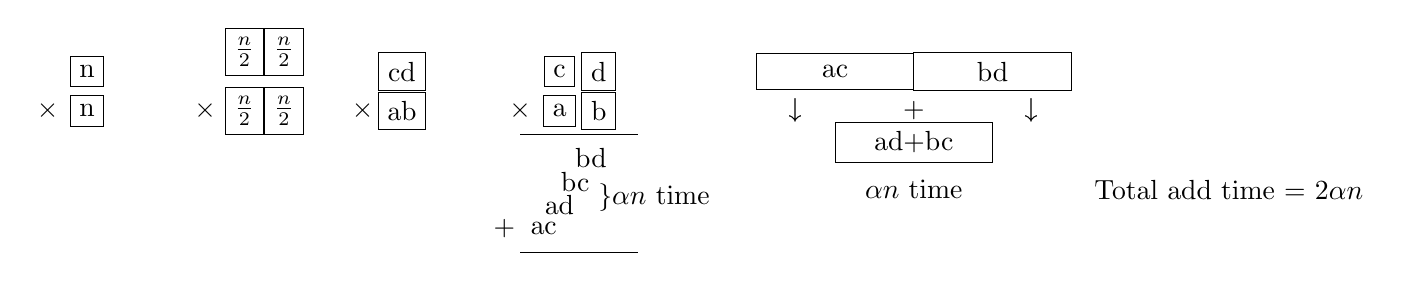
\begin{tikzpicture}
    \node[draw] at (0.5,0) {n};
    \node at (0,0) {$\times$};
    \node[draw] at (0.5,0.5) {n};

    \node[draw] at (2.5,0) {$\frac{n}{2}$};
    \node[draw] at (3,0) {$\frac{n}{2}$};
    \node at (2,0) {$\times$};
    \node[draw] at (2.5,0.75) {$\frac{n}{2}$};
    \node[draw] at (3,0.75) {$\frac{n}{2}$};

    \node[draw] at (4.5,0) {ab};
    \node at (4,0) {$\times$};
    \node[draw] at (4.5,0.5) {cd};

    \node[draw] at (6.5,0) {a};
    \node[draw] at (7,0) {b};
    \node at (6,0) {$\times$};
    \node[draw] at (6.5,0.5) {c};
    \node[draw] at (7,0.5) {d};
    \draw(6,-0.3) -- (7.5,-0.3);
    \node at (6.9,-0.6) {bd};
    \node at (6.7,-0.9) {bc};
    \node at (6.5,-1.2) {ad};
    \node at (7.7,-1.1) {\textbraceright $\alpha n$ time};
    \node at (6.3,-1.5) {ac};
    \node at (5.8,-1.5) {+};
    \draw(6,-1.8) -- (7.5,-1.8);

    \node[draw,minimum width = 2cm, minimum height = 0.45cm] at (10,0.5) {ac};
    \node[draw,minimum width = 2cm] at (12,0.5) {bd};
    \node at (9.5,0) {\textdownarrow};
    \node at (11,0) {+};
    \node at (12.5,0) {\textdownarrow};
    \node[draw,minimum width = 2cm] at (11,-0.4) {ad+bc};
    % \node at (9.5,-1) {$\frac{n}{2}$};
    % \node at (12.5,-1) {$\frac{n}{2}$};
    \node at (11,-1) {$\alpha n$ time};
    \node at (15,-1) {Total add time = $2\alpha n$};
\end{tikzpicture}

$ac$ is an n digit number, as are $ad$, $bc$, $bd$. When adding, $bd$ is not shifted, but $ad$, and $bc$ are shifted by $\frac{n}{2}$ digits, and $ac$ is shifted by n digits.
Since there's no overlap for $ac$ and $bd$, you can add them simply by concatenation.
$ad + bc$ takes $\alpha n$ time. That value plus the center (overlapping) segment of $ac+bd$ is also $\alpha n$.


So without writing out the algorithm: $M(n) = 4M\left( \frac{n}{2} \right)+2\alpha n$ which gives us a nice recursion to work on. Let's assume the time to multiply in the base case is $\mu$. The base case is when both of our numbers are 1 digit long $M(1) = \mu$.

\begin{tikzpicture}
    \Tree [.$2\alpha n$ $\cdots$ $\cdots$ $\cdots$ [.$2\alpha\frac{n}{2}$ $\cdots$ $\cdots$ $\cdots$
        [.$\cdots$ $\cdots$ $\cdots$ $\cdots$ [.$2\alpha\frac{n}{2^k}$ $\mu$ $\mu$ $\mu$ $\mu$ ]]]]
        \node[draw] at (4,0) {$4^0(2\alpha n)$};
        \node[draw] at (5,-1) {$4^1(2\alpha \frac{n}{2})$};
        \node[draw] at (6,-2) {$\vdots$};
        \node[draw] at (8,-3) {$4^{k}(2\alpha \frac{n}{2^{k}})$};
        \node[draw] at (8,-4) {$4^{{\lg(n)}}\mu$};
\end{tikzpicture}

Which is fun, I'm having fun.

\begin{align*}
    \text{comparisons} &= \s{i=0}{\lg(n)-1} (4^i (2\alpha\frac{n}{2^i}) ) + 4^{\lg(n)}\mu \\
    &=2\alpha n \s{i=0}{\lg n-1}\frac{4^i}{2^i} \cdots\\
    &=2\alpha n \s{i=0}{\lg n-1}{2^i} \cdots\\
    &=2\alpha n \left( 2^{\lg n -1 +1} -1 \right) & & \text{geometric series} \\
    &=2\alpha n \left( n-1 \right) \cdots\\
    &\cdots & n^{\lg 4} \mu \\
    &\cdots & n^2 \mu \\
    &= 2\alpha \left( n^2 -n \right)+\mu n^2
\end{align*}

We're doing $n^2$ multiplications and $n^2$ additions, so our application of
recursion didn't improve the running time of our algorithm. There's a better
way!

\subsection{Better Multiplication}

Because of the distributive law $(a+b)(c+d) = ac + ad + bc + bd$. So we can use this property to improve the fast multiplication algorithm.
This will let us replace 1 recursive multiplications with 1 new addition and 1 subtraction, as we shall see.
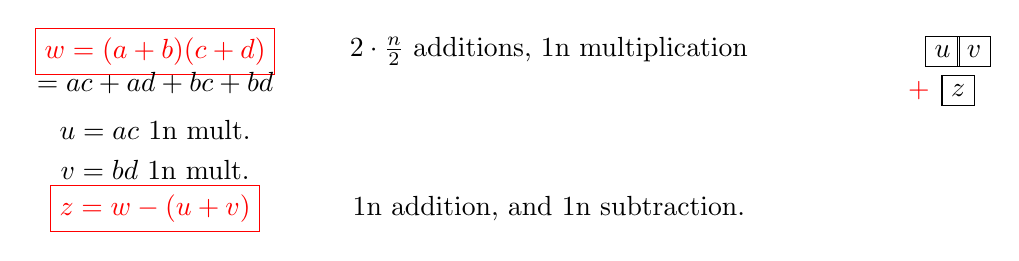
\begin{tikzpicture}
    \node[draw, color=red] at (0,0) {$w=(a+b)(c+d)$};
    \node at (5,0) {$2\cdot\frac{n}{2}$ additions, 1n multiplication};
    \node at (0,-0.4) {$=ac+ad+bc+bd$};
    \node at  (0,-1) {$u=ac$ 1n mult.};
    \node at (0,-1.5) {$v=bd$ 1n mult.};
    \node[draw, color=red] at (0,-2) {$z=w-(u+v)$};
    \node at (5,-2) {1n addition, and 1n subtraction. };
    \node[draw] at (10,0) {$u$};
    \node[draw] at (10.4,0) {$v$};
    \node[draw] at (10.2,-0.5) {$z$};
    \node[color=red] at (9.7,-0.5) {$+$};
\end{tikzpicture}



By the same logic as the earlier multiplication algorithm, $ac$ and $bd$ are
shifted by n bits, and can be concatenated.  Let $w=(a+b)(c+d)$, and $z = w
-(ac + bd) = (ad+bc)$ so to calculate $z$ takes 3 Multiplications, 3 additions
and 1 subtraction. Let's treat the subtraction as an addition, 4 additions.
As such, the recursion for this algorithm is $T(n) = 3T\left( \frac{n}{2} \right)+4\alpha n, T(1) = \mu$.

\begin{align*}
    \s{i=0}{\lg n-1} 3^i \left( 4\alpha \frac{n}{2^i} \right) + 3^{\lg n}\mu &= 4\alpha n \sum \frac{3^i}{2^i} &+n^{\lg 3}\mu \\
    &= 4\alpha n \cdot \frac{{\left(\frac{3}{2} \right)}^{\lg n -1 +1}-1}{\frac{3}{2}-1} &\vdots\\
    &= 4\alpha n \cdot \frac{{\left(\frac{3}{2} \right)}^{\lg n }-1}{\frac{1}{2}} \\
    &= 8\alpha n \left[ n^{\lg \left( \frac{3}{2} \right)}-1 \right]\\
    &= 8\alpha n \left[ n^{\lg 3 - \lg 2}-1 \right]\\
    &= 8\alpha n \left[ \frac{n^{\lg 3}}{n^{\lg 2}}-1 \right]\\
    &= 8\alpha n \left[ \frac{n^{\lg 3}}{n}-1 \right]\\
    &= 8\alpha \left[ {n^{\lg 3}} -n \right] + n^{\lg 3}\mu\\
    &\approx {n^{\lg 3}}\left[ 8\alpha +\mu \right] \\
    &\approx {n^{1.57}}\left[ 8\alpha +\mu \right] \\
\end{align*}

This is $O(n^{1.57})$, a better result than the previous algorithm.


 % ███████                                          ██                     ████     ████                     ██
% ░██░░░░██                                        ░░                     ░██░██   ██░██                    ░██
% ░██   ░██   █████   █████  ██   ██ ██████  ██████ ██  ██████  ███████   ░██░░██ ██ ░██  ██████    ██████ ██████  █████  ██████
% ░███████   ██░░░██ ██░░░██░██  ░██░░██░░█ ██░░░░ ░██ ██░░░░██░░██░░░██  ░██ ░░███  ░██ ░░░░░░██  ██░░░░ ░░░██░  ██░░░██░░██░░█
% ░██░░░██  ░███████░██  ░░ ░██  ░██ ░██ ░ ░░█████ ░██░██   ░██ ░██  ░██  ░██  ░░█   ░██  ███████ ░░█████   ░██  ░███████ ░██ ░
% ░██  ░░██ ░██░░░░ ░██   ██░██  ░██ ░██    ░░░░░██░██░██   ░██ ░██  ░██  ░██   ░    ░██ ██░░░░██  ░░░░░██  ░██  ░██░░░░  ░██
% ░██   ░░██░░██████░░█████ ░░██████░███    ██████ ░██░░██████  ███  ░██  ░██        ░██░░████████ ██████   ░░██ ░░██████░███
% ░░     ░░  ░░░░░░  ░░░░░   ░░░░░░ ░░░    ░░░░░░  ░░  ░░░░░░  ░░░   ░░   ░░         ░░  ░░░░░░░░ ░░░░░░     ░░   ░░░░░░ ░░░
 % ████████                                      ██
% ░██░░░░░                                      ░██
% ░██        ██████  ██████ ██████████  ██   ██ ░██  ██████
% ░███████  ██░░░░██░░██░░█░░██░░██░░██░██  ░██ ░██ ░░░░░░██
% ░██░░░░  ░██   ░██ ░██ ░  ░██ ░██ ░██░██  ░██ ░██  ███████
% ░██      ░██   ░██ ░██    ░██ ░██ ░██░██  ░██ ░██ ██░░░░██
% ░██      ░░██████ ░███    ███ ░██ ░██░░██████ ███░░████████
% ░░        ░░░░░░  ░░░    ░░░  ░░  ░░  ░░░░░░ ░░░  ░░░░░░░░
\section{Recursion Master Formula}
$$ T(n) = aT(\frac{n}{b}) + cn^d, \; T(1)=f$$

Kruskal claims this is a better formula than the master theorem in the book, easier to use and more applicable.
Let's solve using tree method.

\begin{tikzpicture}
    \Tree [.$cn^d$ $\cdots$ $\cdots$ $\cdots$ [.$c\frac{n}{b}^d$ $\cdots$ $\cdots$ $\cdots$
        [.$c\frac{n}{b^2}^d$ $\cdots$ $\cdots$ $\cdots$
            [.$\cdots$ $\cdots$ $\cdots$ $\cdots$ [.$c\frac{n}{b^{n-1}}^d$ $f$ $f$ $f$ $f$ ]]]]]
        \node at (9,1) {num rows};
        \node at (11,1) {sum};
        \node[draw] at (9,0) {$1$};
        \node[draw] at (9,-1) {$a$};
        \node[draw] at (9,-2) {$a^2$};
        \node[draw] at (9,-4) {$a^{n-1}$};
        \node[draw] at (9,-5) {$a^n$};
        \node at (10,-3) {$\vdots$};
        \node[draw] at (11,0) {$cn^d$};
        \node[draw] at (11,-1) {$ac(\frac{n}{b})^d$};
        \node[draw] at (11,-2) {$a^2c(\frac{n}{b^2})^d$};
        \node[draw] at (11,-4) {$a^{n-1}c(\frac{n}{b^{n-1}})^d$};
        \node[draw] at (11,-5) {$fa^{\log_b n}$};
\end{tikzpicture}

You will get $\log_b n$ levels, the branching factor is a.

\begin{align*}
    \s{i=0}{\log_b n-1} a^i c {(\frac{n}{b^i})}^d &= cn^d \s{i=0}{\log_b n-1}\frac{a^i}{{b^i}^d} &+ fn^{\log_b a} \\
    &= cn^d \s{i=0}{\log_b n-1}\frac{a^i}{{b^d}^i} &+ \vdots\\
    &= cn^d \s{i=0}{\log_b n-1}{\left(  \frac{a}{b^d}\right)}^i \\
    &= cn^d \left(\frac{{(\frac{a}{b^d})}^{\log_b n}-1}{\frac{a}{b^d}-1}\right) \\
    &=cn^d \left( \f{n^{\log_b (\frac{a}{b^d})} -1 }{\frac{a}{b^d}-1 } \right) \\
    &=cn^d \left( \f{n^{\log_b {a} -\log_b{b^d}} -1 }{\frac{a}{b^d}-1 } \right) \\
    &=cn^d \left( \f{n^{\log_b {a} -d} -1 }{\frac{a}{b^d}-1 } \right) \\
    &= \f{cn^{\log_b {a}} -cn^d }{\frac{a}{b^d}-1 } +\vdots \\
    &=\frac{cn^{\log_b a}}{\frac{a}{b^d}-1} - \frac{cn^d}{\frac{a}{b^d}-1} + fn^{\log_b a} \\
    &=\left( \frac{c}{\frac{a}{b^d}-1}+f \right)\cdot{n^{\log_b a}} - \frac{cn^d}{\frac{a}{b^d}-1} \\
\end{align*}

This formula can't apply to the situation when the value of a geometric sum
would be 1. The geometric sum isn't applicable in that case. SO this equation
isn't applicable when $a=b^d$, we need a special case. When the r term = 1, a
geometric series becomes a simple summation of 1, thus in this case if $a=b^d$
the formula becomes $cn^d \log_b n + fn^{\log_b a}$.

In the special case of merge sort, we drop the constant -1 from the non
recursion part of the term, and apply the special case, then we repeat the
process with the n dropped, and add the two results.

\begin{align*}
    a\ne b^d && \left( \frac{c}{\frac{a}{b^d}-1}+f \right)\cdot{n^{\log_b a}} - \frac{cn^d}{\frac{a}{b^d}-1} \\\\
    a= b^d && cn^d \log_b n + fn^{\log_b a}
\end{align*}

The relative sizes of these constant factors will overwhelm in differing circumstances.
\begin{align*}
    a > b^d \rightarrow & T(n) \approx \left( \frac{c}{\frac{a}{b^d}-1}+f \right)\cdot n^{\log_b a}  &= \Theta (n^{\log_b a})\\\\
    a < b^d \rightarrow & T(n) \approx \frac{cn^d}{1-\frac{a}{b^d}} &= \Theta (n^d) \\\\
    a = b^d \rightarrow & T(n) \approx cn^d \log_b n \;\;\;\; \text{because $d = \log_b a$} &= \Theta (n^d(\log_b n))\\\\
\end{align*}

\subsection{Applying to known algorithms}
\subsubsection{Multiplication}
\begin{align*}
    T(n)&=4T(\frac{n}{2})+2\alpha n , T(1)=\mu \\
    &a=4,b=2,c=2\alpha,d=1,f=\mu \\
    &\left( \frac{2\alpha}{2-1}+\mu \right)n^{\lg 4} - \frac{2\alpha n}{2-1} \\
    &=\left( 2\alpha+\mu \right)n^2 -2\alpha n \approx \Theta (n^{2}) \\
    &=2\alpha\left( n^2 -n \right)+\mu n^2 \\
    &\approx \Theta (n^{2})
\end{align*}
\subsubsection{Better Multiplication}
\begin{align*}
    T(n)&=3T(\frac{n}{2})+4\alpha n , T(1)=\mu \\
    &a=3,b=2,c=4\alpha,d=1,f=\mu \\
    &\left( \frac{4\alpha}{\frac{3}{2}-1}+\mu \right)n^{\lg 3} - \frac{4\alpha n}{\frac{3}{2}-1} \\
    &=\left( 8\alpha+\mu \right)n^{1.57}-8\alpha n \approx \Theta (n^{1.57}) \\
\end{align*}
\subsubsection{Mergesort}

When we get

\begin{tikzpicture}[sibling distance=200pt]
    \node(a) {$T(n) = 2T(\frac{n}{2}) +n -1, T(1) =0$}
    child{node (l1) {$\text{n term:} \; a=2,b=2,c=1,d=1$}
            child{node (l2) {$a= b^d$}
                child{node (l3){$cn^d \log_b n$}
                    child{node (l4) {$1\cdot n^1 \log_2n = n \lg n$}
                    }
                }
            }
        }
        child{node (r1){$\text{-1 term:} \; a=2,b=2,c=-1,d=0$}
            child{node (r2){$ a\ne b^d$}
                child{node (r3) {$\left( \frac{c}{\frac{a}{b^d}-1}+f \right)\cdot{n^{\log_b a}} - \frac{cn^d}{\frac{a}{b^d}-1}$}
                    child{node (r4) {$\frac{-1}{\frac{2}{2^0 -1}-1}n^{\lg 2} -\frac{-1\cdot n^0}{\frac{2}{2^0}-1}$}
                        child{node (r5) {$ = -n+1$}
    }}}}};
\end{tikzpicture}

\subsubsection{Implementation details}

This gives us the incredible ability to use the constants of the recurrence
into a $\Theta()$ and determine if it will be greater than another algorithm in
constant time.  There's also the Schonhage Strassen algorithm, which is
$\Theta(n\log n \log\log n)$.

In real life, the size of T (1) is the word size of your machine, because the
atomic multiplication is implemented at that level. So our atomic base is
$2^{64}$ for most machines.

 % ██      ██                                                     ██
% ░██     ░██                   ██████                           ░██
% ░██     ░██  █████   ██████  ░██░░░██  ██████  ██████  ██████ ██████
% ░██████████ ██░░░██ ░░░░░░██ ░██  ░██ ██░░░░  ██░░░░██░░██░░█░░░██░
% ░██░░░░░░██░███████  ███████ ░██████ ░░█████ ░██   ░██ ░██ ░   ░██
% ░██     ░██░██░░░░  ██░░░░██ ░██░░░   ░░░░░██░██   ░██ ░██     ░██
% ░██     ░██░░██████░░████████░██      ██████ ░░██████ ░███     ░░██
% ░░      ░░  ░░░░░░  ░░░░░░░░ ░░      ░░░░░░   ░░░░░░  ░░░       ░░
\section{Heapsort}
Created by J.W.J. Williams
Improved by Robert Floyd

\begin{itemize}
    \item Create Heap
    \item Finish
\end{itemize}

\defn[Heap]{A binary tree where every value is larger than its
children. Equivalently its descendants. In this class we require that all
binary trees are full binary trees, where each parent has 2 children.}

\begin{tikzpicture}[centered]
\tikzset{every tree node/.style={draw,circle}, level distance = 2cm, sibling distance = 1cm}
    \Tree[.$100$ [.$90$ [.$80$ $20$ $30$ ] [.$50$ $40$ ] ] [.$70$ $60$ $10$ ]]
\end{tikzpicture}

\subsection{Create Heap}
Turn a tree into a heap.\\
The traditional way to create a heap is to insert at the end of the array and sift up.
Robert Floyd created a better way to create the heap. Treat the tree as a recursive heap:
each parent is the parent to 2 heaps, and sift it from the bottom up. Create heap in left,
create heap on right, then sift root down, and move up a level.

\subsubsection{Heap Creation Analysis}
In a binary tree, most nodes are near bottom, so doing bottom up technique most
work is done near bottom, and because you're near the bottom you don't have far
to go down.  So we take advantage of that fact: Most elements are near the
bottom and don't have far to go.

There are $ \frac{n}{2}$ leaves. Each doing 0 comparisons.

There are $ \frac{n}{4}$ parents of leaves. Each doing 2 comparisons.

There are $ \frac{n}{8}$ grandparents of leaves. Each doing 4 comparisons (2 per level).

There are $ \frac{n}{16}$ greatgrandparents of leaves. Each doing 6 comparisons (2 per level).

\begin{align*}
\frac{n}{2}\cdot0 + \frac{n}{4}\cdot2 + \frac{n}{8}\cdot4 + \frac{n}{16}\cdot6 +\frac{n}{32}\cdot8 + \frac{n}{64}\cdot10 + \cdots \\
= n\cdot\left[ \frac{1}{2} + \frac{2}{4} + \frac{3}{6} + \frac{4}{16} + \frac{5}{32} + \cdots \right]&\l\;\;\;\text{This sum is:} \\
= \frac{1}{2}+\frac{1}{4}+\frac{1}{8}+\frac{1}{16}+\frac{1}{32}+\cdots &= 1 \\
+ \frac{1}{4}+\frac{1}{8}+\frac{1}{16}+\frac{1}{32}+\cdots &= \frac{1}{2} \\
+ \frac{1}{8}+\frac{1}{16}+\frac{1}{32}+\cdots &= \frac{1}{4} \\
+ \frac{1}{16}+\frac{1}{32}+\cdots &=\frac{1}{8} \\
&+\vdots \\
&=2n
\end{align*}

So Heap creation does $\Theta(2n)$ comparisons

\subsection{Finish}
\begin{itemize}
    \item Put root node at the bottom of the array, as it must be the largest element, so
        it will go at the end of the sorted array.
    \item Then take the bottom right hand leaf and move to a tmp space.
    \item Then sift, reordering the tree and put the tmp leaf in its proper spot.
    \item Repeat.
\end{itemize}

Sift comparisons: each level has 2 comparisons, child and tmp. There are
$\approx \lg n $ levels. Total for a sift $\approx 2 \lg n$ This must be done
for each element in the tree, so our heap has an upper bound of $\approx 2n \lg
n$.

But the heap shrinks, each iteration removes an element. So let's sum 0 to n-1
(because we remove an element first before sifting).

\begin{align*}
\s{i=0}{n-1}2 \lg (i+1) &\approx 2\s{i=1}{n}\lg i \\
&=2\left[ \lg 1 + \lg 2 + \lg 3 + \cdots + \lg n \right]\\
&=2 \lg( 1\cdot2\cdot3\cdot\cdots n) \\
&=2 \lg(n!) &\text{Stirling's Formula}\;\;\; n! \approx {\left( \frac{n}{e} \right)}^n \cdot \sqrt{2\pi n} \\
&=2\lg\left[{\left( \frac{n}{e} \right)}^n \cdot \sqrt{2\pi n} \right] \\
&\approx 2\left[ n \lg(\frac{n}{e})+\lg({(2\pi n)}^{\frac{1}{2}}) \right] \\
&= 2\left[ n\left[ \lg n = \lg e \right]+ \frac{1}{2}\lg(2\pi n) \right] \\
&=2n\lg n -2n\lg e + \lg n + \lg(2\pi) \\
&=2n\lg n + O(n)
\end{align*}

This isn't much better, it makes sense that it's not much better than our
conservative guess, because in a full binary tree, half the elements are
leaves. So while the tree shrinks, it doesn't shrink very fast, asymptotically
you're still doing $\Theta(2n\lg n)$ comparisons, plus some linear term.

\subsection{Implementation Details}
Use array to implement tree structure.

\begin{tikzpicture}[centered]
\tikzset{every tree node/.style={draw,circle}, level distance = 2cm, sibling distance = 1cm}
    \Tree[.60 [.30 [.50 20 80 ] [.10 40 ]][.100 70 90 ]];
    \node[draw] at (3,-0.4){tmp};
    \node[vertarray=10] at ++(5,-3)
    (numbers)
    {%
        \strut 60
        \nodepart{two}\strut 30
        \nodepart{three}\strut 100
        \nodepart{four}\strut 50
        \nodepart{five}\strut 10
        \nodepart{six}\strut 70
        \nodepart{seven}\strut 90
        \nodepart{eight}\strut 20
        \nodepart{nine}\strut 80
        \nodepart{ten}\strut 40
    };
    \foreach \Valor [count=\Valori from 1] in {text ,two ,three ,four ,five ,six ,seven ,eight ,nine ,ten }
        \node[anchor=east] at (numbers.\Valor west) {\Valori};

    \node at (9,0) {Node has index $i$};
    \node at (9,-1) {Left child: $2i$};
    \node at (9,-2) {Right child: $2i+1$};
    \node at (9,-3) {Parent: $\lfloor \frac{i}{2} \rfloor$};
\end{tikzpicture}


\textbf{CREATE} The First parent is at index $\lfloor \frac{n}{2} \rfloor$.
Start there and sift down during heap creation. Siblings can be reached by
adding or subtracting 1. Result is a created heap.

\textbf{FINISH} Pop bottom into tmp first, then move heap root into bottom
spot.

\subsection{Optimization}
Why is this result still worse than merge sort? $\Theta(2n\lg n)$ vs
$\Theta(n\lg n)$.  We're comparing tmp against both children and this doubles
our number of comparisons. Instead let's sift the hole left by the root down to
the bottom in $\lg n$ comparisons (1 per level) then put tmp in the hole an sift
it back up into position.

How far will tmp need to go to sift back up and re-form the heap? Not far,
since 1/2 the nodes are in the bottom layer, and 1/4 of the nodes are in the
2nd, etc. It takes 1 comparison to confirm tmp belongs in the bottom layer, 2
to check the 2nd layer up\ldots

$$\frac{1}{2}\cdot1 + \frac{1}{4}\cdot2 + \frac{1}{8}\cdot3 + \frac{1}{16}\cdot4+\cdots = 2$$

Giving 2n comparisons on average. We can further optimize by binary searching
up. This gives Heapsort $ n\lg n + n\lg\lg n= \Theta(n\lg n)$ performance.

\subsection{Pseudocode}
\begin{algorithm}[H]
    \DontPrintSemicolon%
    \SetKwFunction{HPS}{\texttt{Heap\_Sort}}%%
    \SetKwFunction{SIFT}{\texttt{Sift}}%%
    \SetKwProg{Fn}{Function}{is}{end}
    \Fn{\HPS{A,n}}{%
        \tcp*[l]{Create Heap}
        \For{$r=\lfloor \frac{n}{2} \rfloor$ to 1}{%
            \SIFT{r,n,A[r]}\;
        }
        \tcp{Finish Sort}
        \For{$m=n$ To 2}{%
            $s \gets A[m]$\;
            $A[m] \gets A[1]$\;
            \SIFT{1,m-1,s}\;
        }
    }

    \Fn{\SIFT{r,n,s}}{%
        \tcp{r:root index, n:size index, s:sift value, p:parent index, c:child index}
        $p \gets r$ \;
        \While{$2p \le n$}{%
            \eIf{$2p< n$}{%
                \eIf{$A[2p] \ge A[2p+1]$}{%
                    $c\gets 2p$\;
                }{%
                    $c\gets 2p +1$\;
                }
            }{%
                $c\gets 2p$\;
            }
            \eIf{$A[c] > s$}{%
                $A[p] \gets A[c]$\;
                $p \gets c $\;
            }{%
                Break\;
            }
        }
        $A[p] \gets s$\;
    }
    \caption{Heap Sort}
\end{algorithm}

 % ██████                                  ██
% ░█░░░░██                                ░██
% ░█   ░██   ██████  ██   ██ ███████      ░██  ██████
% ░██████   ██░░░░██░██  ░██░░██░░░██  ██████ ██░░░░
% ░█░░░░ ██░██   ░██░██  ░██ ░██  ░██ ██░░░██░░█████
% ░█    ░██░██   ░██░██  ░██ ░██  ░██░██  ░██ ░░░░░██
% ░███████ ░░██████ ░░██████ ███  ░██░░██████ ██████
% ░░░░░░░   ░░░░░░   ░░░░░░ ░░░   ░░  ░░░░░░ ░░░░░░
\section{Finding Bounds to summation functions}
\subsection{Mathematical Preliminaries}
\subsubsection{Geometric Series}
\begin{align*}
    \s{i=0}{\infty}r^{i} &= \frac{1}{1-r} & \text{Infinite Geometric Series}\\
    \s{i=0}{n-1}r^{i} &= \frac{1-r^{n}}{1-r} = \frac{r^n -1}{r-1} & \text{Finite Geometric Series}\\
\end{align*}

\begin{align*}
    \s{i=0}{\infty}i\cdot r^{i} &= \s{i=1}{\infty}i\cdot r^{i} \\
    &= r\cdot\s{i=1}{\infty}i\cdot r^{i-1} \\
    &= r\cdot\s{i=1}{\infty}{\left( \int ir^{i-1} \right)}^{\prime} & \text{sum of derivatives is the derivative of the sum}\\
    &= r\cdot\s{i=1}{\infty}{\left( r^i \right)}^{\prime} \\
    &= r{\left(\s{i=1}{\infty} r^i \right)}^{\prime} \\
    &= r{\left( \frac{1}{1-r}-1 \right)}^{\prime} \\
    &= r\left( \frac{1}{{\left( 1-r \right)}^{2}} \right) \\
    &= \frac{r}{{\left( 1-r \right)}^2}
\end{align*}

How can we check to confirm? We've already calculated the $r=1/2$ case, where the infinite sum is 2.
$$ \frac{\frac{1}{2}}{{\left( 1-\frac{1}{2} \right)}^2} =2$$


Now for the finite series.
\begin{align*}
    \s{i=0}{n-1}i\cdot r^{i} &= \s{i=1}{n-1}i\cdot r^{i} \\
    &= r\cdot\s{i=1}{n-1}i\cdot r^{i-1} \\
    &= r\cdot\s{i=1}{n-1}{\left( \int ir^{i-1} \right)}^{\prime} & \text{sum of derivatives is the derivative of the sum}\\
    &= r\cdot\s{i=1}{n-1}{\left( r^i \right)}^{\prime} \\
    &= r{\left(\s{i=1}{n-1} r^i \right)}^{\prime} \\
    &= r\left[{\left(\s{i=1}{n-1} r^i \right)}^{\prime}\right] \\
    &= r\left[{\left(\frac{r^n-1}{r-1}-1 \right)}^{\prime}\right] \\
    &= r\left[ \frac{nr^{n-1}(r-1)-(r^n-1)}{{(r-1)}^2} \right] \\
    &= r\left[ \frac{nr^n-nr^{n-1}-r^n+1}{{(r-1)}^2} \right] \\
    &= r\left[ \frac{(n-1)r^n-nr^{n-1}+1}{{(r-1)}^2} \right] \\
    &= \frac{(n-1)r^{n+1}-nr^{n}+r}{{(r-1)}^2} \\
\end{align*}

\subsubsection{Gauss's Sum}
$$\s{i=1}{n} i = \frac{n(n+1)}{2} $$ Without knowing the answer already, we can
see an easy upper bound. If every term is bound by it's largest element it
can't be larger than $n^2$. We can also get a lower bound by flooring everything
to the lowest value of 1, since there are n of them we know that the result must
be larger than n. $ n \le sum\le n^2 $.

Next we can try to split the sum in half and floor both to the lowest term in that series.
\begin{align*}
    SUM &= 1+2+3+4+\cdots +\frac{n}{2} + \frac{n}{2}+1+ \cdots +n \\
    &\ge 1+1+1+1+ \cdots +1 \;\;\; + \;\;\; \frac{n}{2}+1 + \cdots + \frac{n}{2}+1 \\
    &\ge \frac{n}{2} + \frac{n}{2}\left( \frac{n}{2}+1 \right) \\
    &\ge \frac{n}{2}\left[ 1+ \frac{n}{2}+1 \right] \\
    &\ge \frac{n}{2}\left[ \frac{n+4}{2} \right] \\
    &\ge \frac{n^2}{4} +n \\
\end{align*}

\subsubsection{Harmonic Sum}
\begin{align*}
    H_n &= \s{i=1}{n} \frac{1}{i} = 1+1/2 +1/3 + 1/4 + 1/5 + \cdots + 1/n \\
    &\approx \ln n \\
    &\text{We can approximate it using the same} \\
    &\text{technique we applied to the Gaussian Sum}\\
    &\le 1 + [1/2 + 1/2] + [1/4 + 1/4 + 1/4 + 1/4] + \cdots \\
    &= 1 + 1 + 1 + \cdots + 1 &\text{num ones = num  groups} \\
    &= \s{i=0}{k-1} 2^i =n \\
    &\text{k is the number of groups. The number of} \\
    &\text{items per group, summed, which must sum to n} \\
    &= 2^k -1 =n \\
    &= 2^k = n+1 \\
    &= k= \lg (n+1) \\
    H_n &\le \lg (n+1) \\
\end{align*}

\subsection{Using continuous math to solve discrete math}

Assume a function that's bounded from m to n the sum of areas in discrete terms is bounded by the integral of some function.
$$\int_{m-1}^n f(x) dx \le \s{i=m}{n} f(i) \le \int_{m}^{n+1} f(x) dx$$ Provided $f(x)$ is increasing.

$$\int_{m}^{n+1} f(x) dx \le \s{i=m}{n} f(i) \le \int_{m-1}^{n} f(x) dx$$ Provided $f(x)$ is decreasing.

\subsubsection{Gauss's Sum}
\begin{align*}
    &\int_{m-1}^n x dx &\le \s{i=m}{n} i &\le \int_{m}^{n+1} x dx \\
    &= \frac{x^2}{2} \Big|_0^n  &&= \frac{n^2}{2} \Big|_i^{n+1} \\
    &= \frac{n^2}{2} -\frac{0^2}{2}  &&= \frac{{(n+1)}^2}{2} -\frac{1^2}{2} \\
    &= \frac{n^2}{2}-0  &&= \frac{n^2+2n+1}{2} -\frac{1}{2} \\
    &= \frac{n^2}{2}  &&= \frac{n^2+2n}{2}  \\
    &= \frac{n^2}{2}  &&= \frac{n(n+2)}{2}
\end{align*}


\subsubsection{Harmonic Sum}
\begin{align*}
    &\int_{m}^{n+1} \frac{1}{x} dx &\le \s{i=m}{n} \frac{1}{i} &\le \int_{m-1}^{n} \frac{1}{x} dx \\
    &\le \ln x \Big|_1^{n+1} &&= \ln(x) \Big|_0^n \\
    &\le \ln (n+1) -\ln(1) &&= \ln(n) -\ln 0 \\
    &\le \ln (n+1) - 0 &&= \ln(n) - (-\infty) \\
    &\le \ln (n+1)  &&= \ln n +\infty \\
    &&&\le +\infty\\
    \intertext{Less than infinity isn't helpful. Let's avoid it by removing the 1 term from the sum, so we don't integrate 0 to 1 for ln x} \\
    &&&\le 1+ \int_{1}^{n} f(x) dx \\
    &&&\le 1+ \ln(x) \Big|_1^n \\
    &&&\le 1+ \ln n - \ln 1 \\
    &&&\le 1+ \ln n -0 \\
    &&&\le \ln(n) + 1 \\
\end{align*}


   % ███████               ██                  ████     ██            ██               ██   ██
  % ██░░░░░██             ░██                 ░██░██   ░██           ░██              ░██  ░░
 % ██     ░░██ ██████     ░██  █████  ██████  ░██░░██  ░██  ██████  ██████  ██████   ██████ ██  ██████  ███████
% ░██      ░██░░██░░█  ██████ ██░░░██░░██░░█  ░██ ░░██ ░██ ██░░░░██░░░██░  ░░░░░░██ ░░░██░ ░██ ██░░░░██░░██░░░██
% ░██      ░██ ░██ ░  ██░░░██░███████ ░██ ░   ░██  ░░██░██░██   ░██  ░██    ███████   ░██  ░██░██   ░██ ░██  ░██
% ░░██     ██  ░██   ░██  ░██░██░░░░  ░██     ░██   ░░████░██   ░██  ░██   ██░░░░██   ░██  ░██░██   ░██ ░██  ░██
 % ░░███████  ░███   ░░██████░░██████░███     ░██    ░░███░░██████   ░░██ ░░████████  ░░██ ░██░░██████  ███  ░██
  % ░░░░░░░   ░░░     ░░░░░░  ░░░░░░ ░░░      ░░      ░░░  ░░░░░░     ░░   ░░░░░░░░    ░░  ░░  ░░░░░░  ░░░   ░░
\section{Order Notation}
Did you know that some algorithms can be faster than others? It's true!

\url{https://en.wikipedia.org/wiki/Time_complexity}
\begin{center}
    \begin{tabular}{lll}
        Name                 & Running time (T(n))        & Examples of running times        \\ \toprule
        Constant             & $ O(1)           $         & 10                               \\ \midrule
        Iterated logarithmic & $ O(\log^* n)      $       & \\ \midrule
        Log-logarithmic      & $ O(\log \log n)   $       & \\ \midrule
        Logarithmic          & $ O(\log n) $              & $ \log n, \log(n^2)$             \\ \midrule
        Polylogarithmic      & $ poly(\log n) $           & $ (\log n)^2  $                  \\ \midrule
        Fractional power     & $ O(n^c) where 0 < c < 1 $ & $ n^{1/2}, n^{2/3}$              \\ \midrule
        Linear               & $ O(n) $                   & $ n$                             \\ \midrule
        N log star n         & $ O(n \log^* n) $          & $   $                            \\ \midrule
        Linearithmic         & $ O(n \log n)$             & $  n \log n, \log n! $           \\ \midrule
        Quadratic            & $ O(n^2) $                 & $  n^2 $                         \\ \midrule
        Cubic                & $ O(n^3) $                 & $  n^3 $                         \\ \midrule
        Polynomial           & $ 2^{O(\log n)} = poly(n)$ & $  n, n\log n, n^{10} $          \\ \midrule
        Quasi-polynomial     & $ 2^{poly(\log n)} $       & $  n^{\log \log n}, n^{log n}$   \\ \midrule
        Exponential (with
        Linear exponent)     & $ 2^{O(n)} $               & $  1.1^n, 10^n $                 \\ \midrule
        Exponential          & $ 2^{poly(n)} $            & $   2^n, 2^{n^2}  $              \\ \midrule
        Factorial            & $ O(n!) $                  & $  n!$                           \\ \midrule
        Double exponential   & $ 2^{2^{poly(n)}} $        & $  2^{2^n}$                    \\
        \bottomrule
    \end{tabular}
\end{center}

\begin{align*}
    \text{Example:} \;\;\;\;\;\;\;\;\;
    &17n^3 +24n^2 -6n +8 \\ %\approx \Theta(n^2) \\
    =& 17n^3 + O(n^2) \\
    =& 17n^3 + o(n^3) \\
    \approx& 17n^3 \\
    =& \Theta{n^3}
\end{align*}

Order notation can hide simple truths like a large constant in a lower order
term that can seriously affect the running time for small n.  Little o means
the function is always less than what's in the bounds. $o(n^3)$ could be
$O(n^{2.9998})$ which could throw off all of our calculations.

\begin{center}
\begin{tabular}{cc}
    Equivalence Function & Order Set\\ \toprule
    $=$ & $\Theta$ \\ \midrule
    $\le$ & $O$ \\ \midrule
    $\ge$ & $\Omega$ \\ \midrule
    $<$ & o \\ \midrule
    $>$ & $\omega$ \\
\end{tabular}
\end{center}


\begin{align*}
    \text{Informally}\;\;\; & f(n) = \Theta(g(n))  \\
    & \lim_{n\ar \infty}\frac{f(n)}{g(n)}= c > 0 \\
    & \lim_{n \ar \infty}\frac{7n^2 +3n -8}{4n^2 +20n +4}=\frac{7}{4}
\end{align*}


\begin{align*}
    \lim_{n \ar \infty} \frac{f(n)}{g(n)} = c \ge 0\lar   f(n) &\in O(g(n))     \\
    \lim_{n \ar \infty} \frac{g(n)}{f(n)} = c \le 0\lar   f(n) &\in \Omega(g(n))\\
    \lim_{n \ar \infty} \frac{f(n)}{g(n)} =0       \lar   f(n) &\in o(g(n))     \\
    \lim_{n \ar \infty} \frac{g(n)}{f(n)} =0       \lar   f(n) &\in \omega(g(n))\\
\end{align*}

What about non-polynomial functions? Like $f(n) = n^2 \cdot(10+\sin (n))$ The
book has a non-limiting approach which gives us a nice way of addressing
oscillating functions.

To a first approximation you can do plain algebra using Theta notation.  $2^{\Theta n^2}\cdot 2^{\Theta n^3}= 2^{\Theta n^2 + \Theta n^3}$.

What's faster? $n^{\lg n} \text{or} {(\lg n)}^n$

Exponentials grow much faster than polynomials. How do we state that formally?
$$n^a = o(b^n) \text{ for } a\ge 0, b>1$$
$${(\log n)}^a = o(n^b) \;\; b>0$$

$${(\log\log n)}^a = o({(\log n)}^b) $$

\begin{align*}
    n^{\lg n } \;\;&?\;\; {(\lg n)}^n \\
    (\lg n)(\lg n) &?\;\; n(\lg\lg n) \\
    {(\lg n)}^2 \;\;&?\;\; n(\lg\lg n) \\
\end{align*}

Polylogs grow slower than polynomials





\end{document}
